\section{Interaktions-Seite [M]}
\setauthor{Fabian Maar}

Bei der Implementierung der Interaktions-Seite, ist es darum gegangen, eine möglichst benutzerfreundliche Besucheransicht der vorhandenen Ausstellungen zu erstellen. 

\subsection{Verbindung der Interaktions-Seite mit der Landing-Page
}
Vorerst muss darauf geachtet werden, dass wenn der*die Benutzer*in eine Ausstellung, die er*sie besuchen möchte, auswählt, auch auf die richtige weitergeleitet wird. Dabei hilft das Routing mit Parametern (siehe Routingparameter \ref{Routingparameter}). Jede Ausstellung besitzt eine eigene ID. Diese ID wird beim auswählen einer Ausstellung in die URL geschrieben, um zu identifizieren zu können, welche Ausstellung im Moment besucht wird. Anhand dieser Informationen werden die Ausstellungsstücke vom Server abgefragt und mit der Logik, die im Kapitel Konfiguration der Ausstellung \ref{Konfigurationstool} beschrieben wird, richtig in den Raum geladen und platziert.

\subsection{Bewegung im dreidimensionalen Raum}
\label{controls}
Um sich im Ausstellungsraum bewegen zu können, ist es nötig, den Besuchern*innen eine entsprechende Fortbewegungsmöglichkeit zu bieten. Three.js implementiert diese Funktion mittels Controls. Im Endeffekt ändert sich die Position und Rotation der Kamera durch Benutzereingaben. Die wesentlichsten Controls in Three.js sind

\begin{itemize}
    \item DragControls - Der*die Nutzer*in kann sich mittels DragNDrop Interaktionen fortbewegen \cite{DragControls}
    \item FirstPersonControls - Der*die Nutzer*in bewegt sich wie in einem Videospiel mit den Tasten W, A, S und D fort. Dabei ist es möglich, das Blickfeld über die Maus zu steuern. \cite{FirstPersonControls}
    \item OrbitControls - Der*die Nutzer*in kann mittels linker Maustaste um ein bestimmtes Ziel kreisen. Durch die rechte Maustaste kann dieses Ziel geändert werden. \cite{OrbitControls}
    \item TransformControls - Den Nutzer*innen ist es möglich ein Objekt, ähnlich wie bei 3D-Modellierungs-Programme, durch Anfasser zu positionieren, skalieren und rotieren. \cite{TransformControls}
    \item PointerLockControls - Diese Art von Controls funktioniert ähnlich wie FirstPersonControls. Hierbei werden ebenfalls die Tasten W, A, S, D benutzt, um sich fortzubewegen. Dabei wird die Maus verwendet, um sich umzuschauen. Jedoch kann die Maussteuerung durch einen Pointer-Lock gesperrt werden.\cite{PointerLockControls}
\end{itemize}


Die beste Wahl für die Fortbewegung in der Ansicht der Erstellung eines Ausstellungsraumes, waren die OrbitControls. Sie eignen sich besonders, da die Benutzer*innen einen guten und schnellen Überblick über den gesamten Raum erhalten.
Die Controls werden initialisiert, indem die Kamera angegeben wird, die gesteuert werden soll und das HTML-Element, welches für die Event-Listener (sieh Event-Listener \ref{txt:glos:event-listener}) benutzt wird.

\begin{lstlisting}[caption={OrbitControls initialisieren},language=TypeScript]
    this.controls = new OrbitControls(this.camera,this.renderer.domElement)
    \end{lstlisting}

Für die Bewegung der Besucher*innen in einem Ausstellungsraum kamen die FirstPersonControls und die PointerLockControls in Frage. Auch wenn sie im Grunde sehr ähnlich sind, besitzen sie verschiedene Vor- und Nachteile. Daher wurden im Entwicklungsprozess beide Varianten getestet und sich für die Bessere entschieden:

\subsubsection{Vor- und Nachteile der FirstPersonControls}

Die FirstPersonControls bieten eine einfache Einbindung in das Programm. Das bedeutet, die Logik des Bewegens muss nicht erst ausprogrammiert werden. Dabei ist es direkt möglich, sich entweder durch die Tasten W, A, S, D, den Pfeiltasten oder durch Linksklick und Rechtsklick fortzusetzen. Außerdem bieten diese Controls einige Konfigurationsmöglichkeiten mehr als die PointerLockControls. Jedoch funktioniert die Maussteuerung nicht gleich, wie sie bei First Person Spiele und Anwendungen üblich ist. Die Kamera dreht sich automatisch in die Richtung weiter, in welche die Maus hinzeigt. Dabei wird die Rotationsgeschwindigkeit von der Position der Maus bestimmt. Je weiter sich die Maus am Bildschirmrand befindet, desto schneller dreht sich die Kamera. Dies mag für viele Benutzer*innen vorerst ein ungewohntes Gefühl sein.

\subsubsection{Implementierung der FirstPersonControls}
Zu Beginn werden neue Controls initialisiert, indem die Kamera angegeben wird, die gesteuert werden soll und das HTML-Element, welches für die Event-Listener(sieh Event-Listener \ref{txt:glos:event-listener}) benutzt wird. 

\begin{lstlisting}[caption={FirstPersonControls initialisieren},language=TypeScript]
    this.controls = new FirstPersonControls(this.camera, this.renderer.domElement)
    \end{lstlisting}

Anschließend werden die Controls wie gewünscht konfiguriert. Spezifische Konfigurationsmöglichkeiten sind: 

\begin{itemize}
    \item activeLook - bestimmt ob die Maussteuerung aktiviert sein soll oder nicht
    \item autoForward - bestimmt, ob sich die Kamera automatisch vorwärts bewegen soll oder nicht. Diese Einstellung ist bei den Controls der 3D-Ausstellung deaktiviert.
    \item constrainVertical, verticalMin und verticalMax - grenzen das vertikale Blickfeld ein
    \item heightMin, heightMax und heightSpeed - werden benutzt um die Bewegungsgeschwindigkeit im Zusammenhang mit der Kamerahöhe zu ändern
    \item lookVertical - bestimmt, ob es möglich ist sich vertikal umzuschauen. Diese Einstellung ist bei den Controls der 3D-Ausstellung deaktiviert.
    \item lookSpeed - gibt an mit welcher Geschwindigkeit sich der*die Benutzer*in umschauen kann
    \item movementSpeed - gibt an mit welcher Geschwindigkeit sich der*die Benutzer*in fortbewegen kann
\end{itemize}
\cite{FirstPersonControls}

\subsubsection{Vor- und Nachteile der PointerLockControls}

Die PointerLockControls bieten, im Gegensatz zu den FirstPersonControls, eine realistische und gewohnte Maussteuerung. Dabei stoppt die Kamera jedes mal an der aktuellen Position, wenn der*die Benutzer*in nicht mit der Maus interagiert. Zudem können die Controls schnellstens durch ein Attribut ge- und entsperrt werden. Jedoch ist es nicht möglich, im entsperrten Zustand mit der Maus zu interagieren. Das bedeutet, Benutzer*innen können sie sich entweder im Ausstellungsraum fortbewegen oder mit einem Ausstellungsstück interagieren, jedoch nicht beides gleichzeitig. Außerdem kommt man viel zu einfach in den gesperrten Zustand, zum Beispiel durch das Drücken der Escape-Taste, das Wechseln vom Browser in ein anderes Programm oder beim Wechseln des Browser-Tabs.  

\subsubsection{Implementierung der PointerLockControls}

Die PointerLockControls bieten, im Gegensatz zu den FirstPersonControls, eine realistische und gewohnte Maussteuerung. Dabei stoppt die Kamera jedes mal an der aktuellen Position, wenn der*die Benutzer*in nicht mit der Maus interagiert. Zudem können die Controls schnellstens durch ein Attribut ge- und entsperrt werden. Jedoch ist es nicht möglich, im entsperrten Zustand mit der Maus zu interagieren. Das bedeutet, Benutzer*innen können sie sich entweder im Ausstellungsraum fortbewegen oder mit einem Ausstellungsstück interagieren, jedoch nicht beides gleichzeitig. Außerdem kommt man viel zu einfach in den gesperrten Zustand, zum Beispiel durch das Drücken der Escape-Taste, das Wechseln vom Browser in ein anderes Programm oder beim Wechseln des Browser-Tabs. 

Zu Beginn werden neue Controls gleich wie bei den FirstPersonControls initialisiert, indem die zu verwendende Kamera und ein HTML-Element zugewiesen werden.
\begin{lstlisting}[caption={PointerLockControls initialisieren},language=TypeScript]
    this.controlsVisitor = new PointerLockControls(this.camera, this.renderer.domElement)
    \end{lstlisting}

Um sich fortbewegen zu können, muss anders wie bei den FirstpPersonControls, die Logik dafür implementiert werden: 

\begin{lstlisting}[caption={Logik der PointerLockControls},language=TypeScript]
    this.onKeyDown = (event: KeyboardEvent) => {
        switch (event.code) {
          case 'KeyW':
            this.controlsVisitor?.moveForward(2)
            break
          case 'KeyA':
            this.controlsVisitor?.moveRight(-2)
            break
          case 'KeyS':
            this.controlsVisitor?.moveForward(-2)
            break
          case 'KeyD':
            this.controlsVisitor?.moveRight(2)
            break
        }
       }
       document.addEventListener('keydown', this.onKeyDown, false)
    \end{lstlisting}

Um die Maussteuerung zu aktivieren müssen außerdem die Controls entsperrt werden:

\begin{lstlisting}[caption={Controls entsperren},language=TypeScript]
    this.controlsVisitor.lock()
    \end{lstlisting}

Auch kann zusätzlich die Geschwindigkeit geändert werden, die angibt, wie schnell sich ein Benutzer im Raum umschauen kann. Zusätzlich kann der horizontale Kamerawinkel konfiguriert werden.

\subsubsection{Fazit}
Da die FirstPersonControls mehr Konfigurations und Interaktionsmöglichkeiten mit den Ausstellungsstücken bieten, wurde für die Fortbewegung als Besucher*in einer Ausstellung diese Art von Controls verwendet.

\cite{PointerLockControls}

\subsection{ThreeJS Clock}
\label{Clock}

Um die im vorherigen Kapitel erwähnten Controls zu updaten, werden sie in der Animations-Schleife (siehe Rendering in ThreeJs \ref{lst:impl:animationloop}) wie folgt aufgerufen: 

\begin{lstlisting}[caption={Controls updaten},language=TypeScript]
    
animate = () => {
    //..
     this.controls?.update(this.clock.getDelta())
    //..}

    \end{lstlisting}

Dabei überprüft die Update-Funktion, welche aktuellen Benutzereingaben betätigt worden sind, um gleichzeitig und flüssig, diese am Bildschirm des*der Benutzers*in anzuzeigen. Dies funktioniert, indem die Position der Kamera zu einem gewissen Zeitpunkt abgefragt wird. Um den aktuellen Zeitpunkt zu erhalten, wird ein Clock-Objekt verwendet. Dieses Clock-Objekt besitzt die Methode getDelta(), um die Sekunden zu erhalten, die vergangen sind, seit die Clock gestartet wurde oder die Methode getDelta() aufgerufen wurde. Außerdem startet die Methode getDelta() die Uhr, falls sie dies noch nicht bereits getan hat. Dadurch können jegliche Updates, die unter anderem durch den*der Benutzer*in, an der Szene vorgenommen worden sind, identifiziert und ausgewertet werden.

\cite{ThreeJsClock}

\subsection{Border-Collision}
Um den Benutzern*innen ein möglichst realistisches Gefühl für die Ausstellung zu geben, ist es wichtig, den Ausstellungsraum authentisch zu gestalten. Daher ist der Raum durch Wände abgegrenzt, wodurch es nicht mehr möglich ist, sich über den Raum hinaus zu bewegen. Um eine Kollision mit der Wand zu berechnen, gibt es durch die Three.js Bibliothek einige Möglichkeiten.


\subsection{Bounding Box}
Der erste Ansatz der Umsetzung war das Erstellen einer Bounding Box. Dabei kann zwischen zwei verschiedenen Arten unterschieden werden. 

\begin{itemize}
    \item Axis Aligned Bounding Box (AABB)
    \newline
    Zum einen werden Axis Aligned Bounding Box verwendet, um eine Box rund um das 3D-Objekt zu erstellen, die sich nicht an die Rotation des Objekts anpasst.
    \item Oriented Bounding Box (OBB)
    \newline
    Die Oriented Bounding Box funktioniert im Endeffekt gleich, unterscheidet sich aber darin, dass sie sich an die Achsen des Objekts anpasst
    
    Da sich die Bounding Boxen jedoch über den ganzen 3D-Raum erstrecken, wird eine Kollision direkt berechnet, nachdem der*die Benutzer*in den Raum betritt. Da sich die Bounding Boxen nicht an jede einzelne Wand anpassen konnten, musste ein anderer Lösungsweg gefunden werden.
\end{itemize}
\begin{figure}
    \centering
    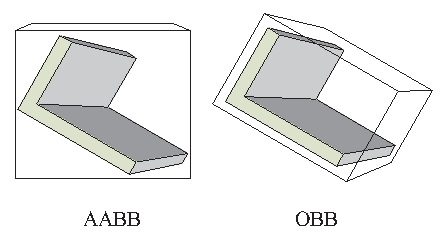
\includegraphics[scale=0.65]{pics/aabb_obb.png}
    \caption{Der Unterschied zwischen AABB und OBB \cite{AABBandOBBPicture}}
    \label{fig:impl:aabb_obb}
\end{figure}


\subsubsection{Zweiter Ansatz}
Um eine Veränderung der Position des*der Benutzers*in festzustellen, muss die Veränderung der Kameraposition evaluiert werden.Bei der Initialisierung der Kamera wird eine Kopie erstellt. In der Animate-Funktion wird eine Veränderung der Kamera überprüft, indem die Positionen der Kamera mit der Kopie verglichen werden. Die Kamera nimmt dabei immer eine neue Position ein, wenn sich der*die Benutzer*in im Raum bewegt, während die Kopie dabei die alte Position der Kamera einnimmt. Jedes Mal wenn eine Veränderung geschieht, wird überprüft, ob die Kamera mit der Wand kollidiert. Dies geschieht, indem ein Raycast mit den Positionen der Kamera und der Kopie initialisiert wird. 
     
\subsubsection{Far und Near}
Die Attribute Far und Near werden dafür verwendet, um die Objekte, die im Ray liegen, einzugrenzen. Dies wird durch die Methode des Clippings realisiert (siehe Clipping \ref{clipping}). Dabei können die Werte nicht negativ sein und der Far-Wert muss größer als der Near-Wert sein. Um die Kollision erst direkt am Ursprungsort, im Falle der Kamera, des Rays zu berechnen, wird der Far-Wert auf 100 gesetzt.
   	
Nachdem der Raycast (siehe Raycast \ref{impl:int:raycasting}) Referenz korrekt initialisiert und angewandt wurde, muss bei einer Berührung mit der Wand nur noch richtig damit umgegangen werden. Dabei wird die Bewegung des Benutzers gestoppt. Um diese auch wieder zu starten, muss sich der*die Benutzer*in weg von der Wand begeben. Überprüft wird dies nach jeder Benutzer*inneneingabe mit einem Event-Listener. Falls nach dieser keine Berührung mehr mit einer Wand besteht, wird die Bewegung fortgesetzt und der*die Besucher*in kann sich wieder frei im Raum bewegen.


\subsection{Interaktion}
Als Besucher*in einer Ausstellung soll es möglich sein, benutzerfreundlich mit den Ausstellungsstücken zu interagieren. Dazu zählen die Markierung des ausgewählten Ausstellungsstückes und die dazugehörige Detailansicht. 

\subsubsection{Raycasting}
\label{impl:int:raycasting}
Raycasting ist eine der wichtigsten Komponenten, um mit einem 3D-Modell interagieren zu können. Wie das Konzept des Raycastings funktioniert, wurde bereits im Kapitel Rendering erklärt (siehe Rendering \ref{impl:rend:raycasting}) Referenz. Three.js besitzt seinen ganz eigenen Raycaster. Er wird vor allem dafür genutzt, um herauszufinden, auf welchem 3D-Objekt sich der Mauszeiger aktuell befindet. Es gibt mehrere Möglichkeiten einen Raycaster zu erstellen. Zum einen kann er normal über einen Constructor initialisiert werden. Dabei wird angegeben, von welchen Koordinaten der Ray ausgeht und in welche Richtung er geschickt wird. Andererseits kann ein Raycaster direkt von einer schon existierenden Kamera einen Ray wegschicken. Dafür wird die Methode .setFromCamera aufgerufen, wo die Koordinaten des Mauszeigers und die zugehörige Kamera angegeben werden. Alle vom Ray getroffenen 3D-Objekte werden Intersections genannt. Diese 3D-Objekte können durch die Methode intersectsObject ausgelesen und in ein Array und gespeichert werden.

\subsubsection{Hover-Effekt}
Um zu erkennen, welches Ausstellungsstück momentan vom Mauszeiger gehovert wird, wird ein solcher Raycaster verwendet. Zu Beginn werden die Koordinaten des Mauszeigers in einem zweidimensionalen Vektor gespeichert. Ein Event-Listener wird hierbei jedes Mal aufgerufen, wenn sich der Mauszeiger bewegt. Darin können dann die kalkulierten Positionen des Mauszeigers dem Vektor zugewiesen werden.

\begin{lstlisting}[caption={Aktuelle Koordinaten des Mauszeigers einem 2D-Vektor zuweisen},language=TypeScript]
    
    pointer = new THREE.Vector2()

    window.addEventListener( 'pointermove', (event: PointerEvent) => {
            // calculate pointer position in normalized device coordinates
            // (-1 to +1) for both components
            this.pointer.x = ( event.clientX / window.innerWidth ) * 2 - 1
            this.pointer.y = - ( event.clientY / window.innerHeight ) * 2 + 1
            this.hoverExhibit()
          });
    
    
        \end{lstlisting}

Anschließend wird ein neuer Raycaster mit dem zweidimensionalen Vektor und der bereits existierenden Kamera erstellt. 

\begin{lstlisting}[caption={Neuen Raycaster anlegen},language=TypeScript]
    
    this.raycaster.setFromCamera(this.pointer, this.camera! )
    
\end{lstlisting}

Daraufhin können alle 3D-Objekte die vom Ray getroffen wurden, in einem Array gespeichert werden.

\begin{lstlisting}[caption={Intersected Objects auslesen},language=TypeScript]
    
    const intersects=this.raycaster.intersectObjects(this.scene.children)
    
\end{lstlisting}

Um die Ausstellungsstücke farblich zu umranden, müssen sie zunächst ausgelesen werden. Dabei iteriert eine for-Schleife durch alle Ausstellungsstücke durch. Um zu erkennen, ob ein Intersect ein Ausstellungsstück ist, werden die jeweiligen IDs miteinander verglichen. Um dem 3D-Objekt einen Bloom-Effekt, also einen farbigen Schein als Umrandung, hinzuzufügen, wird das Konzept des Post-Processings verwendet.

\begin{lstlisting}[caption={Intersects als Ausstellungsstück identifizieren},language=TypeScript]
    
    for (let value of values) {


    if (value.uuid != null) {
    if (value.uuid == intersects[0].object.parent?.parent?.uuid || value.uuid == intersects[0].object.uuid) {

        const object = this.scene.getObjectByProperty('uuid', value.uuid);
        const renderPass = new RenderPass( this.scene, this.camera! );
        this.composer = new EffectComposer(this.renderer!)
        this.composer.addPass( renderPass );
    
        const outlinePass = new OutlinePass( new THREE.Vector2( window.innerWidth, window.innerHeight ), this.scene, this.camera! );
        this.composer.addPass( outlinePass );


        this.addSelectedObjects(object!);


        outlinePass.selectedObjects = this.selectedObjects;
      }
    }
  }

\end{lstlisting}

Um den Effekt wieder zu entfernen, da ein anderes Ausstellungsstück gehovert wurde, wird ein Array verwendet, das das alte Objekt herausgibt und das neue hinzufügt.

\begin{lstlisting}[caption={Hover-effekt wieder entfernen},language=TypeScript]
    
addSelectedObjects( object: Object3D ){
    this.selectedObjects = [];
    this.selectedObjects.push(object)
  }
    
\end{lstlisting}

\subsubsection{Postprocessing}
Post-Processing ist eine Render-Methode, die zum Beispiel für Anti-Aliasing, Tiefenschärfe und andere 3D-Effekte benutzt wird. Dabei wird zuerst die Szene mit den gewünschten 3D-Objekten gerendert und im Speicher der Grafikkarte zwischengespeichert. Anschließend werden beim Post-Processing verschiedene Filter angewandt, diese gerendert und dem*der Benutzer*in angezeigt. In Three.js wird dafür ein EffectComposer verwendet. Dieser enthält ein Array von allen Effekten, die angewandt werden und dann mittels WebGL-Renderer in einer bestimmten Reihenfolge gerendert werden. Für die visuelle Anzeige sind Post-Processing-Passes zuständig. Zu Beginn wird ein RenderPass angelegt, der die zugehörige Kamera und Szene rendert. Anschließend können verschiedene Effekt-Passes, wie zum Beispiel der OutlinePass oder der GlitchPass, hinzugefügt werden. \cite{PostProcessing}

\subsubsection{Detailansicht}

Um beim Klicken auf ein Ausstellungsstück zur gewünschten Detailansicht zu kommen, wird ebenfalls ein Raycaster benutzt. Die Logik funktioniert fast gleich wie beim Hover-Effekt. Jedoch werden die Koordinaten des Mauszeigers nur bei jedem Mausklick aktualisiert. Gleich wie beim Hover-Effekt, wird das Array der Ausstellungsstücke mit einer For-Schleife durchiteriert. Dadurch kann identifiziert werden welches Ausstellungsstück von dem*der Benutzer*in angeklickt wurde. Dabei werden die Informationen des Ausstellungsstückes an ein Dialogfenster geschickt, welches als Detailansicht fungiert.  

\begin{lstlisting}[caption={identifizieren des geklickten Ausstellungsstückes},language=TypeScript]
    
  for (let value of values) {
    if (value.uuid == intersects[0].object.parent?.parent?.uuid) {
      if (value.uuid != null) {
        const object = this.scene.getObjectByProperty('uuid', value.uuid);
        this.objectDescription = value.description
        this.objectTitle = value.title
        this.objectUrl = value.exhibit_url
        this.openDialog('1000ms', '300ms')
      }
  }
}

\end{lstlisting}

Geöffnet wird das Dialogfenster über eine eigene openDialog-Funktion. Dabei wird eine neue Instanz von einem Dialogfenster angelegt, welches Angular-Material verwendet. Dabei wird angegeben, welche Größe und Breite das Fenster haben soll. Auch wird festgelegt, wie schnell die Animation zum Öffnen und Schließen abläuft. Um die Daten des Ausstellungsstücks auch im Dialogfenster zur Verfügung zu stellen, werden diese beim initialisieren angegeben.

\begin{lstlisting}[caption={initialisieren des Dialogfensters},language=TypeScript]
    
  openDialog(enterAnimationDuration: string, Fertige Fertige LandingLandingexitAnimationDuration: string): void {
    const dialogRef = this.dialog.open(ExhibitDialog, {
       maxWidth: '100vw',
       maxHeight: '50vh',
       width: '100%',
       height: '100%',
       data: {description: this.objectDescription, title: this.objectTitle, objectUrl: this.objectUrl},
       enterAnimationDuration,
       exitAnimationDuration,
     });
//..
}
\end{lstlisting}

Wenn sich der*die Benutzer*in in der Detailansicht befindet, soll die Animation im Hintergrund gestoppt werden. Dies erfolgt durch die Methode \emph{cancelAnimationFrame}, wodurch die Animations-Schleife angehalten wird. Um den aktuellen Zeitpunkt zu erhalten, zu dem die Animation gestoppt wird, wird die \emph{requestAnimationFrame} Methode verwendet. Diese wird in der Animations-Schleife aufgerufen und dabei wird der aktuelle Frame der Animation zurück geliefert. Um sich nicht mehr weiter in der Ausstellung fortbewegen zu können, wird die Clock (siehe Clock \ref{Clock}) gestoppt, die für die Three.js Controls benötigt wird. Nachdem der*die Benutzer*in das Dialogfenster wieder schließt, wird die Animations-Schleife und die Clock wieder fortgesetzt. 

Ein Problem ist, dass der Raycast nicht automatisch deaktiviert wird, wenn man sich in der Detailansicht befindet. Das bedeutet, dass es dem*der Benutzer*in weiterhin möglich ist, im Hintergrund weitere Instanzen des Dialogfensters zu öffnen. Dies führt zu einer Duplizierung der Detailansicht. Daher wird anhand einer Boolean-Variable festgestellt, ob das Dialogfenster bereits geöffnet ist, um den Raycast zu deaktivieren. 

\begin{lstlisting}[caption={Öffnen und Schließen des Dialogfensters},language=TypeScript]
  openDialog(enterAnimationDuration: string, exitAnimationDuration: string): void {
      //..
      this.dialogOpen = true
      cancelAnimationFrame(this.animationid!)
      this.clock.stop()
  
      dialogRef.afterClosed().subscribe(r => {
        this.dialogOpen = false
        this.animate()
        this.clock.start()
      })
    }
\end{lstlisting}

Das Dialogfenster ist eine eigene Angular-Komponente. Im Konstruktor der Komponente werden die Daten des Ausstellungsstückes injiziert, um es anschließend in einer detaillierten Ansicht zu rendern. Dabei werden eigens für die Detailansicht ein neuer Canvas angelegt, eine neue 3D-Szene gerendert und mittels Animations-Schleife neue Orbit-Controls (siehe Controls \ref{controls}) initialisiert. Dadurch kann das 3D-Objekt frei betrachtet werden. Falls beim Konfigurieren der Ausstellung, dem Ausstellungsstück, eine Beschreibung mitgegeben wurde, wird diese in diesem Dialogfenster angezeigt.

  \begin{lstlisting}[caption={Constructor-Injection in der Dialog Komponente},language=TypeScript]
    constructor(@Inject(MAT_DIALOG_DATA) public data: any, public dialogRef: MatDialogRef<ExhibitDialog>) {}

  \end{lstlisting}

\subsubsection{Navigation}
Benutzer*innen können ebenfalls direkt in der Detailansicht zwischen den einzelnen Ausstellungsstücken wechseln. Dadurch müssen Benutzer*innen die Detailansicht nicht ständig verlassen, wodurch sich Zeit und Benutzereingaben gespart werden können. Außerdem kann dadurch eine Ausstellung, ähnlich wie bei dem Programm PowerPoint, gut für präsentierende Zwecke genutzt werden. 



\subsection{Erledigte Userstories [L]}
In dem Entwicklungsprozess der Interatkionsmethoden wurden folgende Userstories vollendet:

\begin{compactenum}       
  \item Als User*in möchte ich mich auf verschiedene Arten in der Ausstellung bewegen können. Akzeptanzkriterien:
  \begin{compactitem}
      \item Per Slideshow (über den Vorwärts/Rückwärts-Pfeil zu nächstem Ausstellungsstück springen)
      \item Per Touch / Click (Google Maps Street View, NavigationMesh in Three.js https://github.com/donmccurdy/three-pathfinding)
  \end{compactitem}
  \item  Als User*in möchte ich auf das Ausstellungsstück klicken können, um weitere Informationen (z.B.: Titel, Künstler, Jahr, …) zu erhalten. Akzeptanzkriterien:
  \begin{compactitem}
      \item größere Ansicht des Ausstellungsstücks wird vergrößert angezeigt
      \item Nähere Details zum Ausstellungsstück, wie Titel, Künstler, Jahr, usw.
  \end{compactitem}
\end{compactenum}